\documentclass[11pt]{article} 
%\documentclass[11pt,dvipdfm]{article} 

\usepackage{deauthor,times,graphicx} 
\usepackage[hidelinks]{hyperref}
\usepackage{tcolorbox}

\graphicspath{{istvan/}} 
\usepackage{xpatch}
\makeatletter

\makeatletter


\begin{document}

\title{The Glass Half Full: Using Programmable \\ Hardware Accelerators in Analytics
}
\author{Zsolt Istv\'{a}n\\ \small IMDEA Software Institute, Madrid, Spain\\  \small \{first.lastname@imdea.org\}}

\maketitle

\begin{abstract}
There have been numeorus proposals to accelerate databases using specialized hardware in past years but 
often the opinion of the community is pessimistic: the performance and energy efficiency benefits of 
specialization are seen to be outweighed by the limitations of the proposed solutions and the 
additional complexity of including specialized hardware, such as field programmable gate arrays (FPGAs), 
in servers. Recently, however, as an effect of stagnating CPU performance, server architectures started to incorporate various programmable hardware components, ranging from smart network interface cards, through SSDs with offloading capabilities, to near-CPU accelerators. The availability of heterogeneous hardware brings opportunities
to databases and we make the case that there is cause for optimism. In the light of a shifting hardware landscape 
and emerging analytics workloads, it is time to revisit our stance on hardware acceleration. 

In this paper we highlight several challenges that have traditionally hindered the deployment of hardware acceleration in databases and explain how they have been alleviated or removed altogether by recent research results and the changing hardware landscape. We also highlight that, now that these challenges have been addressed, a new set of questions emerge around the integration of heterogeneous programmable hardware in tomorrow's databases, for which answers can likely be found only in collaboration with researchers from other fields.

\end{abstract}

\section{Introduction}

There is a rich history of projects aiming to specialize computers (or parts of computers) to databases. Notable examples include the Database Machine from the seventies~\cite{banerjee-databasemachine-79}, Gamma~\cite{dewitt-gamma-1990}, the Netezza data appliance~\cite{francesco-netezza-2011}, the Q100 DB processor~\cite{wu-q100-asplos14}, and Oracle Rapid~\cite{agrawal-rapid-17} most recently. These works demonstrate orders of magnitude increase in energy efficiency and better performance thanks to a hardware/software co-design approach. However, CPUs, until very recently, enjoyed a performance scaling in line with Moore's law and the time and effort of designing and delivering specialized hardware was not economical. This changed with the stagnation in CPU performance~\cite{esmaeilzadeh-darksilicon-isca11} and the simultaneous increase in networking speeds in the last decade that has created a clear need for hardware acceleration. 

Initially, the move to the cloud worked against hardware acceleration for databases due to the cloud's reliance on commodity hardware and the need to cater to many different users and applications. Recently, however, new data-intensive workloads emerged in the cloud (most notably machine learning), that suffered from stagnating CPU performance and could benefit from various types of compute or networking acceleration. If we look at today's cloud offering and datacenters, an exciting, heterogeneous landscape emerges: Machine learning workloads in the Google Cloud are accelerated with Tensor Processing Units (TPUs)~\cite{sato-tpu-google17}, increasing energy efficiency by at least an order of magnitude when compared to GPUs. Amazon, Baidu and Huawei all offer Field Programmable Gate Arrays (FPGAs) by the hour in their cloud to users\footnote{At the moment of writing it costs around \$1.65/h to rent an Amazon EC2 F1 instance.} to implement custom accelerators. Microsoft, in project Catapult~\cite{firestone-catapult-nsdi18}, has been deploying FPGAs in the Azure Cloud to accelerate their infrastructure and machine learning pipelines. Furthermore, Intel has been experimenting with including small programmable elements on their Xeon CPUs~\cite{gupta-harp-fpl16} that can be tailored to accelerate different user applications. 

These recent developments mean that multi-purpose programmable hardware accelerators are entering the mainstream and, from the point of view of the database, they can be exploited without having to incur additional deployment costs. Specialized hardware is most often used to accelerate compute-bound operations and the ongoing shift in the analytical database workloads towards machine learning~\cite{mahajan-danafpga-vldb18}\cite{hellerstein-madlib-vldb12}\footnote{For instance, Microsoft SQL Server now includes machine learning plug-ins. \url{https://docs.microsoft.com/en-us/sql/advanced-analytics/what-is-sql-server-machine-learning}} brings significantly more compute-intensive operations than the core SQL operators. What's more, there are proposals for using machine learning methods to replace parts of the decision making and optimization processes inside databases~\cite{kraska-sage-cidr19}. These emerging operators bring new opportunities in hardware acceleration both inside databases and for user workloads. Furthermore, now that hardware acceleration of real-world workloads is economically feasible, new challenges emerge around deep integration of programmable hardware in databases. 


In this paper we make the case that there is cause for optimism, thanks to the two trends mentioned above, namely, datacenters becoming increasingly heterogeneous and workloads opening towards machine learning. These, combined with the state of the art in hardware acceleration for databases, tackle most of the past hindrances of programmable hardware adoption. We will focus on FPGAs as a representative example and discuss how several significant challenges have been alleviated recently. In the final part of this paper we highlight open questions around the topics of resource management and query planning/compilation in the presence of programmable hardware accelerators.


\section{Background}


\subsection{Programmable Hardware in the Datacenter}


The wide range of programmable hardware devices proposed and already deployed in datacenters can be categorized depending on their location with regards to the data source and CPU into three categories (see Figure~\ref{fig:acceleratorlocations}): on-the-side, in data-path and co-processor.

\begin{figure}[h]
\centering
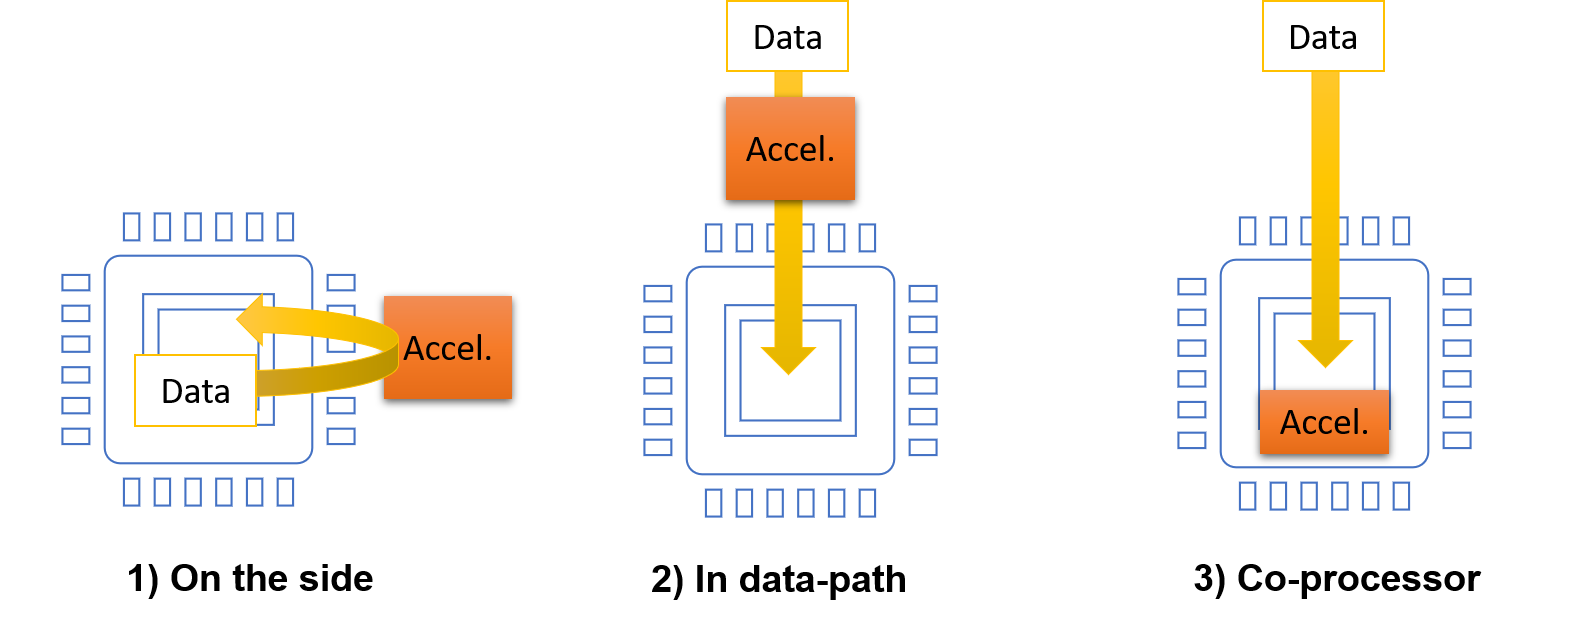
\includegraphics[width=0.75\linewidth]{figs/accelerator-location.png}
\caption{Programmable hardware accelerators can be deployed either as ``on-the-side'' accelerator (e.g., GPUs), as ``in data-path'' accelerator (e.g. smart NICs, smart SSD), or as co-processor (e.g. in Oracle DAX or Intel Xeon+FPGA). \label{fig:acceleratorlocations}}
\end{figure}

The most traditional way we think about accelerators is as being \emph{on-the-side} (Figure~\ref{fig:acceleratorlocations}.1), attached to the processor via an interconnect, for instance PCIe. Importantly, in this deployment scenario the CPU owns the data and explicitly sends it to the accelerator, resulting usually in significant additional latency per operation due to communication latency and data transformation overhead. This encourages offloading operations at large granularity and without requiring back and forth communication between the CPU and the accelerator. GPUs are a common example of this kind of accelerator and were shown to be useful, for instance, to offload LIKE-based string queries~\cite{sitaridi-gpuregex-2016}. There have also been proposals that deploy FPGAs this way for data filtering and decompression, e.g., in the work by Sukhwani et al.~\cite{sukhwani-dbanalyitcs-ieee14}.

Another way of placing acceleration functionality in the architecture is \emph{in data-path} (Figure~\ref{fig:acceleratorlocations}.2). This can be thought of as a generalized version of near-data processing~\cite{oskin-active-ieee98}, and the goal of the accelerator is to filter or transform data at the speed that it is received from the data source. Designs that can't guarantee this could end up slowing down the entire system~\cite{koo-summarizer-micro17}. Much of the research effort in this space has been centered around in-SSD processing~\cite{jo-yoursql-vldb16}\cite{woods-Ibex-vldb14}, but more recently there have been efforts in using RDMA network interface cards (NICs) to accelerate distributed databases~\cite{barthels-join-sigmod15}\cite{dragojevic-farm-debull17}. These NICs are limited to data manipulation acceleration, but there are efforts to make NICs and networking hardware in general more programmable~\cite{bosshart-p4-comrew14}. This will allow offloading in the future complex, application-specific, operations.

The third deployment option, namely, \emph{co-processor} (Figure~\ref{fig:acceleratorlocations}.3), is also becoming increasingly available in the form of CPUs that integrate domain-specific or general-purpose programmable co-processors: The Oracle DAX~\cite{aingaran-dax-hcs16} is an example of the former because it implements database-specific operations, such as data decompression, scan acceleration, comparison-based filtering, on data in the last level cache. Thanks to its specialized nature, it occupies negligible chip space and does not increase the cost of the CPU. As opposed to the DAX, the Intel Xeon+FPGA~\cite{gupta-harp-fpl16} platform offers an FPGA beside the CPU cores for general-purpose acceleration. The FPGA has high bandwidth cache-coherent access to the main memory and can be reprogrammed in different ways. This creates acceleration opportunities without the usual overhead of the on-the-side accelerators.


\subsection{Field Programmable Gate Arrays}

FPGAs are chips that can be programmed to implement arbitrary circuits and historically have been used to prototype and validate designs that would result later in Application-Specific Integrated Circuits (ASICs). They have recently become a target for implementing data processing accelerators in datacenters thanks to their flexibility (their role can change over time, as opposed to an ASIC) and orders of magnitude better energy efficiency than that of traditional CPUs~\cite{teubner-fpgabook-2011}. FPGAs are composed of look-up tables (LUTs), on-chip memory (BRAM) and digital signal processing units (DSPs). All these components can be configured and interconnected flexibly, allowing the programmer to implement custom processing elements (Figure~\ref{fig:insidefpga}). It is not uncommon to have small ARM cores integrated inside the programmable fabric either, e.g., in Xilinx's Zynq product line. 


\begin{figure}[h]
\centering
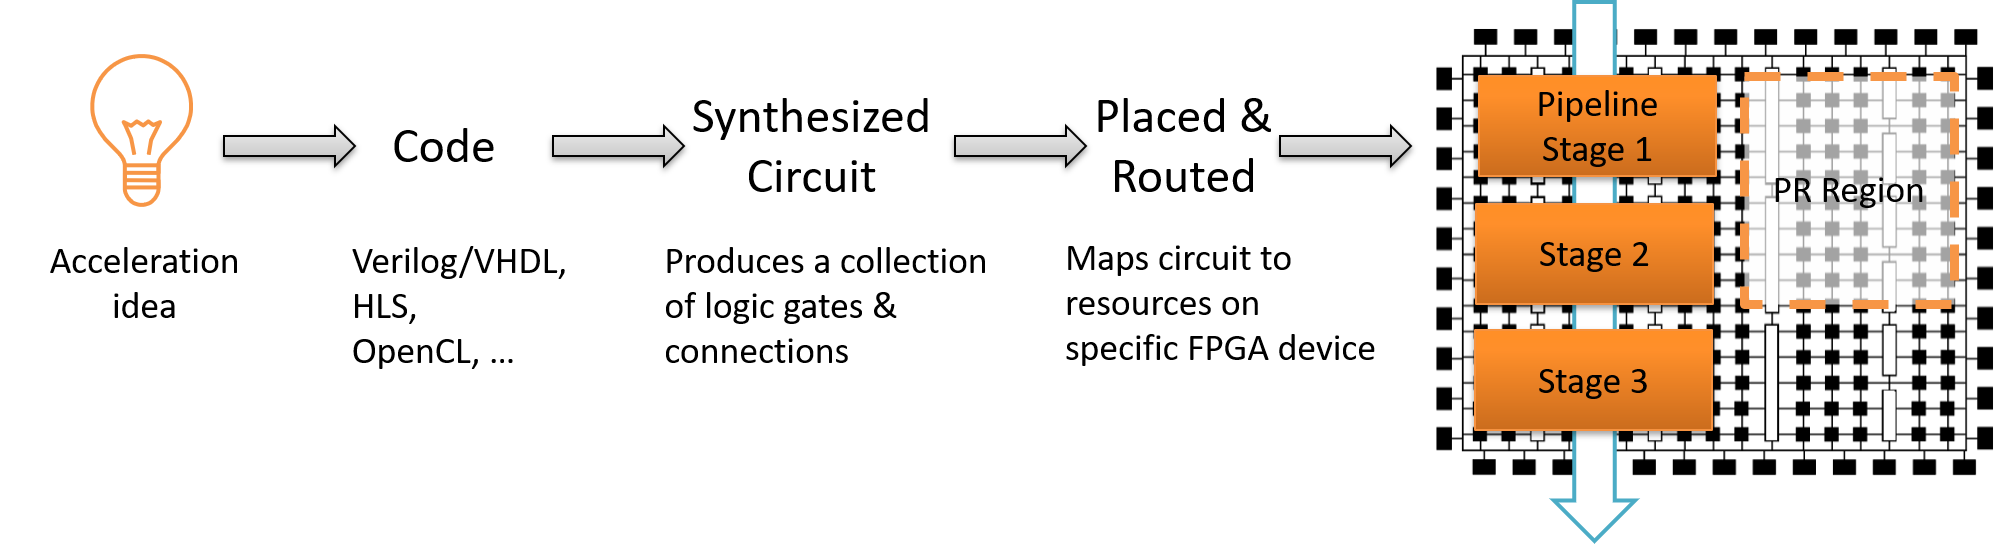
\includegraphics[width=0.9\linewidth]{figs/fpga-internal.PNG}
\vspace{-1em}
\caption{The typical steps of programming FPGAs are shown above. The tools spend most of their time mapping the synthesized circuit onto the FPGA. This is because the chip is composed of many programmable gates and memories that have to be configured and connected together in a 2D space, ensuring that signals can propagate correctly within clock periods.\label{fig:insidefpga}}
\end{figure}


FPGAs offer two types of parallelism: first, pipeline parallelism means that complex functionality can be executed in steps without reducing throughput. The benefit of FPGAs in this context is that the communication between pipeline stages is very efficient thanks to the physical proximity and availability of on-chip memory to construct FIFO buffers. The second type of parallelism that is often exploited on FPGAs is data-parallel execution. This is like SIMD (single instruction multiple data) processing in CPUs, but it can also implement a SPMD (single program multiple data) paradigm if the operations are coarser grained. What makes FPGAs interesting for acceleration is that these two types of parallelism can be combined even inside a single application module to provide both complex processing and scalable throughput.

As Figure~\ref{fig:insidefpga} shows, FPGAs are programmed by synthesizing a circuit from a hardware definition language, such as Verilog or VHLD, and creating a ``bitstream'' for a specific device type that defines the behavior of every logic resource on the chip. This is an expensive step as it requires the tool to lay out the circuit on the ``chip surface'' and define connections and routing of these connections between circuit elements. Since FPGAs have flexible clocking options and the programmer is free to define a target frequency (e.g., 300MHz), the tools have to set up routing such that signals are propagated within the clock periods (which can become impossible with too high frequencies). 

It is also possible to perform partial reconfiguration (PR), meaning that only a portion of the FPGA's resources are reprogrammed (illustrated on the right-hand side of Figure~\ref{fig:insidefpga}). This means that, for instance, in a database use-case a hardware-accelerated operator can be replaced with another one without having to bring the device offline. PR, however, comes with limitations: the regions can only be defined at coarse granularity, their size can't be redefined at runtime and their reprogramming requires milliseconds. 

One important limitation of FPGAs is that all application logic occupies chip space and there is no possibility of ``paging'' code in or out dynamically. This means that the complexity of the operator that is being offloaded is limited by the available logic resources (area) on the FPGA. This also applies to the ``state'' of an algorithm that is often stored as data in the on-chip BRAM memories. These can be accessed in a single clock cycle, but if the data doesn't fit in the available BRAM, high latency off-chip DRAM has to be used. 

\section{Sources of Pessimism}

Many early projects of FPGA-based database acceleration propose deploying them as on-the-side accelerators for row stores~\cite{sukhwani-dbanalyitcs-ieee14}\cite{casper-fpgaacceldb-fccm14}\cite{dennl-sqlaccel-fccm13} and they demonstrate that FPGAs are able to successfully accelerate selection, projection, group-by aggregation, joins and even sorting, by an order of magnitude when compared to MySQL and Postgres, for instance. However, the \textbf{benefits are significantly reduced once one factors in the cost of communication over PCIe and the software overhead} of preparing the data for the FPGA to work on (sometimes pre-parsing, often copying pages). 

In traditional, on-the-side deployments, the high latency communication (microseconds over PCIe) often forces designs to move entire operators onto the FPGA, even if only parts of the operator were a good match for the hardware. This leads to complications, because even though FPGAs excel at parallel and pipelined execution, they behave poorly when an algorithm requires iterative code or has widely branching ``if-then-else'' logic. In the case of the former, CPUs deliver higher performance thanks to their higher clock rates. In the case of the latter, the branching logic needs to be mapped to logic gates that encode all outcomes, resulting in very large circuits. Since the space on the FPGA is limited, the larger circuits result in reduced parallelism, which in turn leads to lower throughput. This means that even though FPGAs could be successful in accelerating the common case of an algorithm, they might not be able to handle corner cases, and in practice this \textbf{leads to uncertainty in the query optimizer or even to wasted work, if an unexpected corner case is encountered during execution}. 

In parallel with accelerator-based efforts, there have been numerous advances in the space of analytical databases. Today, column-oriented databases, such as MonetDB~\cite{boncz-x100-cidr05}, are widely deployed and typically outperform row-oriented ones by at least an order of magnitude and can take advantage of many-core CPUs efficiently. As a result, the \textbf{speedups that FPGAs offer when targeting core SQL operators have shrunk}\footnote{Using specialized hardware can still compete with multi-cores if we factor in energy efficiency (Operations/s/Watt) but in many cases the metric that is of interest is database throughput and response time.} and often are not enough to motivate the additional effort of integrating specialized hardware in the server architecture.

For the above reasons, FPGA-based acceleration ideas are often received with pessimism. However, changes in the hardware available in datacenters and the cloud, as well as the changes in database architecture and user workloads, create novel opportunities for FPGA-based acceleration. In the next section we discuss these in more detail and provide examples of how they can be exploited.







\section{Reasons for Optimism}



\subsection{Changing Architectures}
%Solved challenge 1: data movement overhead -- near-cpu accelerators, capable smartNICs 

With the increasing adoption of distributed architectures for analytical databases, as well as the disaggregation efforts in the datacenter~\cite{klimovic-flash-eurosys16}, there are numerous opportunities for moving computation closer to the data source to reduce the data movement bottlenecks. These bottlenecks arise from the fact that the access bandwidths are higher closer to the data source than over the network/interconnect and they can be eliminated by pushing filtering or similar data reduction operations closer to source. Thus, \textbf{the main goal of accelerators in the data-path is to reduce the amount of data sent to the processor, while maintaining high data access bandwidths.} 


The data source is often (network-attached) flash storage and recent projects, for instance, YourSQL~\cite{jo-yoursql-vldb16}, BlueDBM~\cite{jun-bluedbm-tocs16} and Ibex~\cite{woods-Ibex-vldb14}, show that it is possible to execute SQL operations as the data is moving from storage to processing at high bandwidth. Another use-case that can benefit from data reduction in a similar way is ETL. Recent work~\cite{fang-udp-micro17} has demonstrated that specialized hardware can be used to offer a wide range of ETL operations at high data rate, including: (de)compression, parsing from formats such as CSV or JSON, pattern matching and histogram creation.

In Ibex we deployed an FPGA between an SSD and the CPU, offering several operators that can be plugged into MySQL's query plans. As Figure~\ref{fig:Ibex} shows, these include scans, projection, filtering and group-by aggregation, and were chosen in a way that ensures that processing in hardware will reduce the final data size for most queries. For this reason, Ibex does not accelerate joins, since these would potentially result in larger output than input and slow down the system this way. The rest of the operations are all performed at the rate of the data arriving from storage.


\begin{figure}[h]
\centering
\includegraphics[width=0.7\linewidth]{figs/Ibex.PNG}
\vspace{-1em}
\caption{In Ibex we showcase several operations that can be performed on the data as it is read from storage with the goal of reducing the number of tuples that arrive at the CPU.\label{fig:Ibex}}
\end{figure}

As opposed to on-the-side accelerators, in this space there are two possible options for who ``owns'' the data. In the case of smart SSDs, data is typically managed by the host database~\cite{jo-yoursql-vldb16}\cite{woods-Ibex-vldb14}. In contrast, in the case of distributed storage accessed over the network, it is possible to explore designs where the data is both processed and managed by the specialized hardware device as, for instance, in Caribou~\cite{istvan-caribou-vldb17}\cite{zistvan-diss-2018}, our distributed key-value store that is built using only FPGAs. 

In Caribou, the FPGAs implement, in addition to network line-rate data processing, a hash table data structure and memory allocator necessary for managing large amounts of data, as well as, data replication techniques to ensure that no records are lost or corrupted in case of device failures or network partitions. This results in a high throughput, energy efficient distributed storage layer that, even though is built using FPGAs, can be used as a drop-in replacement for software-based solutions~\cite{zistvan-diss-2018}.



In many ways, in-data-path accelerators provide similar acceleration options as the on-the-side ones because data is still moved over a network (similarly to an interconnect in the case of the latter) that requires processing it in large enough batches to warrant the latency overhead. However, if FPGAs are deployed as co-processors, this overhead is drastically reduced and new opportunities open up, since the latency to the FPGA is in the same order of magnitude as a cross-socket memory access. The Centaur platform~\cite{owaida-centaur-fccm17}, for instance, exposes the FPGA of an Intel Xeon+FPGA platform using an efficient ``hardware thread'' API. As a result, in this co-processor scenario, \textbf{the database can offload functionality as if spawning a parallel thread and the FPGA can be used for processing even just a handful of tuples} -- as we point out in the next subsection, there are emerging use-cases where this low latency acceleration is a game-changer. 

\subsection{Emerging Compute-Intensive Workloads}

%Solved challenge 3: thin margins on core SQL operations -- shift to ML type workloads, DBs becoming more complex themselves, as a sideeffect of CH1 we can now target sub-operator acceleration as well.

The examples in the previous subsection showed how to reduce the data access bottleneck with an in data-path accelerator targeting common SQL operators. It is unclear, however, if this strategy can be applied for co-processors as well.
Modern database engines, that make use of the multi-core CPUs and their wide SIMD units, are rarely compute bound once the data is loaded into main memory. Unless reading data from storage, \textbf{offloading core SQL operators is unlikely to bring orders of magnitudes improvements in performance. There is, however, cause for optimism if we look beyond such operators and in the direction of machine learning}, both training and inference.

A significant portion of machine learning pipelines operate on relational data and the case has been made that there is a benefit in integrating these pipelines directly in the database~\cite{mahajan-danafpga-vldb18}. Furthermore, there is also interest in including such components in the internal modules of the databases~\cite{kraska-sage-cidr19}, to perform optimizations depending on the workload characteristics and the model. Since this could require on-line retraining that, without hardware acceleration, could hurt user throughput significantly, new opportunities open up for FPGAs. Acceleration of training as part of user workloads is being explored, for instance in Dana~\cite{mahajan-danafpga-vldb18}. The iterative and computation-heavy nature of training operators makes them less sensitive to the latency issues introduced by using on-the-side accelerators and therefore could revive the interest in these acceleration platforms. Amazon, for instance, is already offering FPGAs running Xilinx's OpenCL-based compute framework as PCIe-attached accelerators. 

In the ``ML-backed'' database scenario it will also be paramount to be able to take decisions with low latency using learned models -- this further motivates the use of FPGAs. Even though GPUs are a de-facto standard for machine learning acceleration, when it comes to low latency inference, FPGAs can offer benefits since they do not require batching in their processing modules: recent work by Owaida et al.~\cite{owaida-trees-fpl17} and Umuroglu et al.~\cite{umuroglu-finn-fpga17} demonstrates, for instance, how FPGAs can be used very efficiently to accelerate inference using decision trees, respectively, neural networks. 

\subsection{Hybrid Approaches to Acceleration}
\label{sec:hybrid-comp}

Since all functionality, regardless whether used or not, occupies chip space on the FPGA, \textbf{corner cases often can't be efficiently handled in hardware. For this reason, it is important to design accelerators such that they behave predictably even if the particular instance of the problem can't be fully handled.} As we illustrate below with two examples from our work, state of the art solutions overcame such cases by splitting functionality between FPGA and software, such that the part on the FPGA remains beneficial to execution time regardless of the input data contents or distribution. 


\begin{figure}[b]
\centering
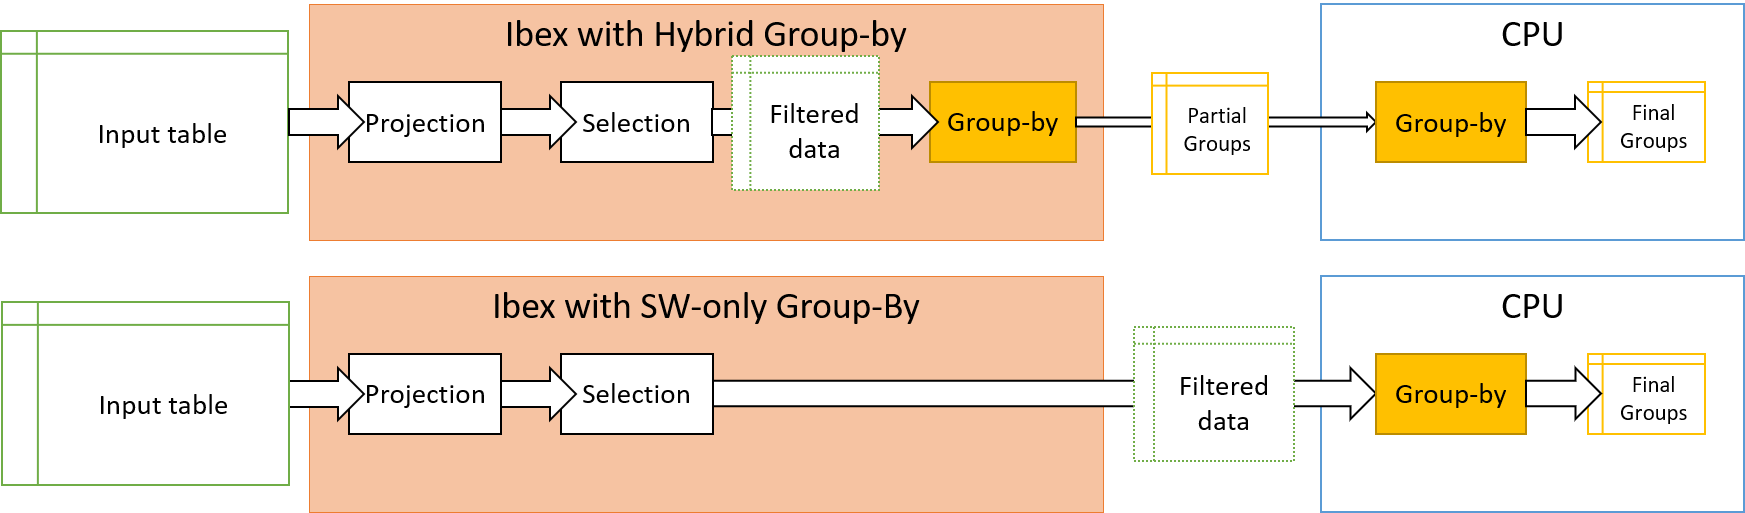
\includegraphics[width=0.9\linewidth]{figs/hybrid-compute.png}
\caption{By implementing operators in a way that allows hybrid computation, the FPGA accelerator can reduce data sizes over the bottleneck connection to the CPU in most cases. In this example of Ibex's group-by operator, if we would choose an ``all or nothing approach'', moving the data to be aggregated to the CPU could become the bottleneck.\label{fig:hybrid-compute}}
\end{figure}


In Ibex~\cite{woods-Ibex-vldb14} we used a hybrid methodology to implement a group-by operator that supports \texttt{min}, \texttt{max}, \texttt{count} and \texttt{sum} (in order to compute \texttt{avg}, we used query rewriting to compute the count and sums). This operator is built around a small hash table that collects the aggregate values. In line with FPGA best-practices, the hash table is of fixed size and is implemented in BRAM. The reason for this is that this way it is possible to guarantee fixed bandwidth operation, regardless of the data contents, because the FPGA doesn't have to pause processing to resize the table. 

Unfortunately, this approach has a drawback: if a query has just one more group than the size of the hash table, the FPGA can't be used -- and this information is often not available up front. We overcome this situation by post-processing the results of the group-by operator on the FPGA in software. The hardware returns results from the group by aggregation unit in a format that allows the database to perform an additional aggregation step without having to apply projections on the tuples or parse them in the first place (see Figure~\ref{fig:hybrid-compute}). If during the hash table operations collisions are encountered that can't be solved, a partial aggregate is evicted from the table and sent to the software post-processor. Once all the data has been processed on the FPGA, the contents of the hash table are sent to the software post-processor to compute the final groups. This results in a behavior where, if all the groups could be computed on the FPGA, the final software step has to perform virtually no work (assuming that the number of resulting groups is significantly smaller than the cardinality of the table), and otherwise the software executes the group by aggregation as if there wasn't any FPGA present (though still benefits from projections and selections).



\begin{figure}[t]
\centering
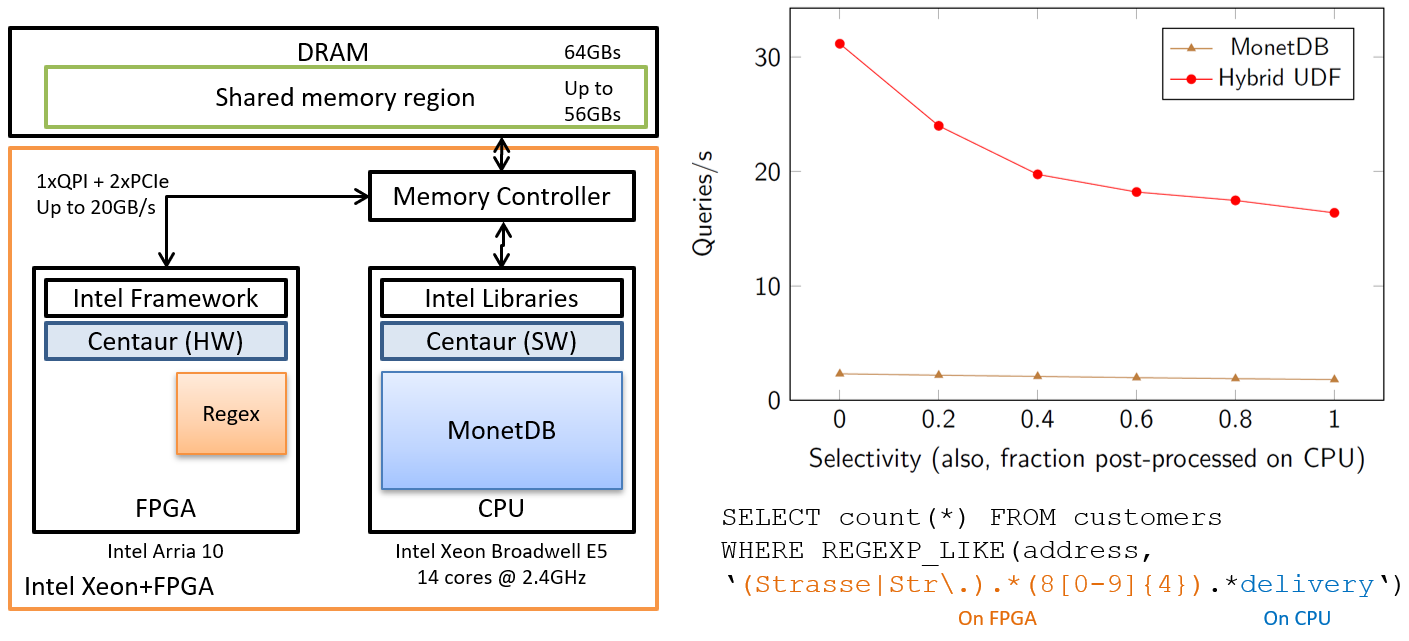
\includegraphics[width=0.9\linewidth]{figs/hybrid-exec.png}
\caption{Even if only part of the regular expression fits on the FPGA it is worth to offload it because the post-processing becomes cheaper, resulting in an overall faster execution.\label{fig:hybrid-regex}}
\end{figure}

The regular expression-based LIKE operator that we implemented in MonetDB~\cite{sidler-regex-sigmod17} running on top of the Intel Xeon+FPGA platform is another example of the hybrid operator methodology. If the expression can't be encoded in its entirety on the FPGA, because, for instance, it contains too many characters (such as the bottom example in Figure~\ref{fig:hybrid-regex}), we cut it at the last possible wildcard and process the first part of the expression on the FPGA and the second part in software. For each string, the FPGA operator returns an index that signifies the end of the location where the regular expression matched the string. The software can pick up processing from this point in case of hybrid processing and match the rest of the expression. In case the entire expression fits on the FPGA, however, the software has no additional work to do. In Figure~\ref{fig:hybrid-regex} we illustrate how, when compared to a single-threaded execution in MonetDB, the hybrid solution is always faster than the software-only one (for more details see~\cite{sidler-regex-sigmod17}). 

One aspect that makes the integration of programmable hardware in databases challenging is the change in the predictability of query runtimes. Therefore, in our work we aim to design circuits whose throughput is not affected by the problem instance they work on. This way the query optimizer can predict the rate at which data will be processed/filtered on the FPGA and with this information it can reliably decide when to offload. One example of such a design is the regular expression module we presented above. Since the overhead of compiling regular expressions to circuits and then performing partial reconfiguration (PR) could take longer than executing an entire query, we took a different approach: we created a ``universal'' automaton that could implement any expression, within some limits on the number of distinct characters to detect and the number of states. Small on-chip memories are used to describe the state machine and the characters of the regular expression, and their contents can be loaded at runtime in nanoseconds. We laid out this state machine as a pipeline, that processes one character per clock cycle, regardless of the contents of the on-chip memories. The conversion from a regular expression written by a user to the configuration parameters is performed in software but is orders of magnitude cheaper than circuit synthesis.


\section{The Road that Lies Ahead}

\subsection{Managing Programmable Hardware}

%\begin{tcolorbox}
\emph{How to best integrate hardware that, even though reprogrammable, will never be as flexible as software?}\\
\emph{Should the operating system/hypervisor control it, or can we build future databases that do this?}
%\end{tcolorbox}
\smallskip

Even though there are efforts in the FPGA community to speed up the process of partial reconfiguration, it is unlikely that the overhead of this operation will ever be as small as that of a software context switch. As a result, databases must find ways to adapt to the idea of running on specialized hardware that, even though, can be reprogrammed, doesn't have the flexibility of software. The main question that needs to be answered in this space is who will ``own'' the acceleration functionality, because this also defines whether the database needs only to be able to compile its queries to take advantage of the accelerators, or whether it could also synthesize fully custom accelerators depending on the workload.

If it is the OS/hypervisor that controls the accelerator, then the database still has to be able to adapt to different underlying hardware acceleration functionality, that will likely be both designed and managed by the infrastructure/cloud provider. In this scenario, the database has to create query plans that take advantage of the specific machine's acceleration opportunities. For this, it is likely that we can reuse techniques that are already present in databases for compiling code for different target CPU features such as SIMD units~\cite{pirk-compiler-cidr19}.

Alternatively, if the database takes full ownership of the accelerator, it will have more responsibility but also greater opportunities. Instead of relying on the cloud provider to design general-purpose acceleration units that might or might not match the database's needs, the database developer can design and synthesize the right ones and integrate them tighter with the database. What's more, the database could even generate and synthesize workload-specific accelerators at runtime.

In DoppioDB~\cite{owaida-centaur-fccm17}\cite{sidler-doppiodb-sigmod17} we explored the case where the database manages the accelerator. The role of the operating system is to set up a basic infrastructure on the FPGA, configuring it with several ``slots'' that can be filled in using partial reconfiguration (we call these slots hardware threads because the interface to them in software is similar to a function call on a new thread). Once the database has started, the FPGA gets access to the process's virtual memory space and the database can explicitly manage what tasks the different slots perform, choosing in our prototype from a small library of available operators. In DoppioDB, instead of focusing only on the usual SQL operators like selection or joins, we began exploring how one could extend what the database is capable of, targeting machine learning type of operators, such as training a model using stochastic gradient descent or running inference with decision trees. This functionality was exposed using a UDF mechanism, but in the future could be integrated much tighter with the database. The research question that emerges is how to populate the hardware operator library and what granularity these operators should have. Recent work by Kara et al.~\cite{kara-join-sigmod17} shows that it is possible to offload sub-operators successfully to the FPGA. However, the identification of generic enough sub-operators that can be deployed on an accelerator and parameterized/composed at runtime remains an open challenge.

\subsection{Compilation/Synthesis for Programmable Hardware}


%\begin{tcolorbox}
\emph{Are there reusable building blocks that would make query compilation easier for programmable hardware?}\\
\emph{Should databases have their own DSLs from which to generate hardware accelerators?}
\smallskip
%\end{tcolorbox}

The second big question is how to express acceleration functionality for database use-cases in an efficient way. As opposed to CPUs or GPUs where the architecture (ISA, caches, etc.) is fixed, in an FPGA it is not. This adds a layer of complexity to the problem of compiling operators, as well as query planning in general. 
Given even just the heterogeneity of modern CPUs and their different SIMD units, there is already a push for databases to incorporate more and more compiler ideas~\cite{pirk-compiler-cidr19}\cite{pirk-voodoo-vldb16}. 

The side effect of bringing more ideas from compilers into databases is that it will likely also be easier to integrate DSLs for hardware accelerators~\cite{sycl2016}\cite{koeplinger-spatial-pldi18}\cite{maxcompiler} into the database. However, many of these solutions are targeting compute kernels written in languages such as OpenCL~\cite{sycl2016}, that are a better fit for HPC and machine learning type functionality than database operations. Therefore, novel ideas are needed that bridge the space between databases and languages/compilers for specialized hardware. One possible direction to explore is related to the design of the Spatial language and compiler~\cite{koeplinger-spatial-pldi18}. Spatial approaches the problem of writing parallel code for accelerators in a way that accounts for the fact that circuits are physically laid out on the chip. Given that query plans are often composed by a set of sub-operators that are parameterized differently to implement, for instance, different join types, these could be an intermediate step between SQL and hardware circuit that allows the database to offload a pipeline of such sub-operators to the FPGA in an automated manner.

Another aspect that makes translating operators to hardware-based accelerators challenging comes from the fact that not all functionality will fit on the device.  This is true regardless whether we target an FPGA, a P4-based switch or SmartNIC, or an ASIC-based solution such as the DAX. Therefore, even if the best case of an operator can be efficiently translated to hardware, corner cases will have to be handled without significantly impacting performance. For this reason, the challenge of compilation is also related to the ideas discussed before around hybrid execution and query planning. Frameworks that compile queries to such platforms will have to provide software-based post-processing functionality to ensure that corner cases are gracefully handled. The challenge in this hybrid computation is to find suitable points where to split the functionality in an automated way.

\section{Conclusion}

In this paper we made the case that the use of specialized hardware in analytical databases has a positive outlook, even though it has been approached pessimistically for a long time. To support this argument, we discussed the past and future challenges of including a specific kind of hardware accelerator, namely FPGAs, in databases. 

To address fears that deploying FPGAs always brings high overheads that reduce their ``raw'' speedup, we highlighted how, in today's distributed database landscape, they can be used to reduce bottlenecks of data movement by positioning them in data-path. Since they can process data at the rate at which it is retrieved from the data source, they never slow down data access, even if there is no opportunity for acceleration. We also discussed the opportunities that novel machine learning workloads bring. Their operators are typically compute bound on CPUs and using FPGAs we can achieve significant speedups even when compared to an entire socket with multiple cores. Finally, to demonstrate that it is possible to design FPGA-based operators that behave gracefully even if the entire functionality of the operator doesn't fit on the device, we discussed two examples from our previous work that implement hybrid computation across FPGA and CPU (a group-by operator and a regular expression matcher).

We also identify two areas in which significant progress has to be made for the inclusion of heterogeneous hardware in databases to become truly widespread. One is finding ways to actively manage the programmable hardware underneath the database, shaping it to workloads using partial reconfiguration and parameterizable circuits. The second question is about finding the right programming primitives for hardware accelerators in the context of database operators, to avoid designing from scratch each new accelerator idea and to allow the database to offload parts of a query more flexibly at runtime. It is unlikely that we can provide answers for both questions only from inside the database community and will have to instead collaborate with researchers working in the areas of operating systems, programming languages and compilers.

\small
\section*{Acknowledgments}

Our cited work and many of the lessons learned are a result of the author's collaboration with current and past members of the Systems Group at ETH Z\"{u}rich, in particular, Gustavo Alonso, David Sidler, Louis Woods and Jana Giceva.


\begin{thebibliography}{10} 
\itemsep=1pt 

\bibitem{banerjee-databasemachine-79} J. Banerjee, D. Hsiao and K. Kannan. \newblock DBC: A Database Computer for Very Large Databases. \newblock \emph{IEEE Transactions on Computers}, 6, pp. 414-429, IEEE, 1979.

\bibitem{dewitt-gamma-1990} D.J. DeWitt, S. Ghandeharizadeh, D.A. Schneider, A. Bricker, H.I. Hsiao, R. Rasmussen. \newblock The Gamma database machine project. \newblock \emph{IEEE Transactions on Knowledge and data engineering}, 2(1), pp. 44-62, 1990.

\bibitem{francesco-netezza-2011} P. Francisco. \newblock The Netezza data appliance architecture: A platform for high performance data warehousing and analytics. \newblock \emph{IBM Red Books}, 2011.

\bibitem{wu-q100-asplos14} L. Wu, A. Lottarini, T.K. Paine, M. Kim, K.A. Ross \newblock Q100: The Architecture and Design of a Database Processing Unit. \newblock \emph{ASPLOS'14}, pp. 255-268, 2014.

\bibitem{agrawal-rapid-17} S.R. Agrawal, S. Idicula, A. Raghavan, E. Vlachos, V. Govindaraju, V. Varadarajan, E. Sedlar et al. \newblock A many-core architecture for in-memory data processing. \newblock \emph{MICRO'17}, pp. 245-258, ACM, 2017.

\bibitem{esmaeilzadeh-darksilicon-isca11} H. Esmaeilzadeh, E. Blem, R.S. Amant, K. Sankaralingam and D. Burger. \newblock Dark silicon and the end of multicore scaling. \newblock \emph{ISCA'11}, pp. 365-376, IEEE, 2011. 

\bibitem{sato-tpu-google17} K. Sato, C. Young, D. Patterson. \newblock An in-depth look at Google’s first Tensor Processing Unit (TPU). \newblock \emph{Google Cloud Big Data and Machine Learning Blog, 12}, 2017.

\bibitem{firestone-catapult-nsdi18} D. Firestone, A. Putnam, S. Mundkur, D. Chiou, A. Dabagh, et al. \newblock Azure Accelerated Networking: SmartNICs in the Public Cloud. \newblock \emph{NSDI'18}, USENIX, 2018.

\bibitem{gupta-harp-fpl16} P.K. Gupta. \newblock Accelerating datacenter workloads. \newblock \emph{FPL'16}, 2016.

\bibitem{mahajan-danafpga-vldb18} D. Mahajan, J.K. Kim, J. Sacks, A. Ardalan, A. Kumar, H. Esmaeilzadeh. \newblock In-RDBMS Hardware Acceleration of Advanced Analytics. \newblock \emph{Proceedings of the VLDB Endowment}, 11(11), 2018.

\bibitem{hellerstein-madlib-vldb12} J.M. Hellerstein, C. Re, F. Schoppmann, D.Z. Wang, E. Fratkin, A. Gorajek, K.S. Ng, C. Welton, X. Feng, K. Li,et al. \newblock The MADlib analytics library: or MAD skills, the SQL. \newblock \emph{PVLDB}, 5(12), pp. 1700–1711, 2012.

\bibitem{kraska-sage-cidr19} T. Kraska, M. Alizadeh, A. Beutel, E. Chi, J. Ding, A. Kristo, V. Nathan, et al. \newblock SageDB: A learned database system. \newblock \emph{CIDR'19}, 2019.

\bibitem{sitaridi-gpuregex-2016} E. Sitaridi, K. Ross. \newblock GPU-accelerated string matching for database applications. \newblock \emph{Proceedings of the VLDB Endowment}, pp. 719-740, 2016.

\bibitem{sukhwani-dbanalyitcs-ieee14} B. Sukhwani, H. Min, M. Thoennes, P. Dube, B. Brezzo, S. Asaad, D.E. Dillenberger. \newblock \emph{Database analytics: A reconfigurable-computing approach}, IEEE Micro, 34(1), pp. 19-29, 2014.

\bibitem{oskin-active-ieee98} M. Oskin, F.T. Chong, T. Sherwood. \newblock Active pages: A computation model for intelligent memory. \newblock \emph{IEEE Computer Society}, Vol. 26, No. 3, pp. 192-203, 1988.

\bibitem{koo-summarizer-micro17} G. Koo, K.K. Matam, H.V. Narra, J. Li, H.W. Tseng, S. Swanson, M. Annavaram. \newblock Summarizer: trading communication with computing near storage. \newblock \emph{MICRO'17}, pp. 219-231, ACM, 2017.

\bibitem{jo-yoursql-vldb16} I. Jo, D.H. Bae, A.S. Yoon, J.U. Kang, S. Cho, D. Lee, J. Jeong. \newblock YourSQL: a high-performance database system leveraging in-storage computing. \newblock \emph{Proceedings of the VLDB Endowment}, 9(12), pp. 924-935, 2016.

\bibitem{woods-Ibex-vldb14} L. Woods, Z. Istvan, G. Alonso. \newblock Ibex: an intelligent storage engine with support for advanced SQL offloading. \newblock \emph{Proceedings of the VLDB Endowment}, 7(11), pp. 963-974, 2014.

\bibitem{jun-bluedbm-tocs16} S.W. Jun, M. Liu, S. Lee, J. Hicks, J. Ankcorn, M. King, S. Xu. \newblock BlueDBM: Distributed Flash Storage for Big Data Analytics. \newblock \emph{ACM TOCS} 34(3), 7, 2016.

\bibitem{barthels-join-sigmod15} C. Barthels, S. Loesing, G. Alonso, D. Kossmann. \newblock Rack-scale in-memory join processing using RDMA. \newblock \emph{SIGMOD'15}, pp. 1463-1475, ACM, 2015.

\bibitem{dragojevic-farm-debull17} A. Dragojevic; D. Narayanan; M. Castro. \newblock RDMA Reads: To Use or Not to Use?. \newblock \emph{IEEE Data Eng. Bull.}, vol. 40, no 1, pp. 3-14, 2017.

\bibitem{bosshart-p4-comrew14} P. Bosshart, D. Daly, G. Gibb, M. Izzard, N. McKeown, J. Rexford, et al. \newblock P4: Programming protocol-independent packet processors. \newblock \emph{ACM SIGCOMM Computer Communication Review}, 44(3), pp. 87-95, 2014.

\bibitem{aingaran-dax-hcs16} K. Aingaran, S. Jairath, D. Lutz. \newblock Software in Silicon in the Oracle SPARC M7 processor. \newblock \emph{Hot Chips Symposium (HCS'16)}, pp. 1-31, IEEE, 2016.

\bibitem{teubner-fpgabook-2011} J. Teubner and L. Woods. \newblock Data processing on FPGAs. \newblock \emph{Synthesis Lectures on Data Management}, 5(2), pp. 1-118, 2011.

\bibitem{casper-fpgaacceldb-fccm14} J. Casper, K. Olukotun. \newblock Hardware acceleration of database operations. \newblock \emph{FPGA'14}, pp. 151-160, ACM, 2014.

\bibitem{dennl-sqlaccel-fccm13} C. Dennl, D. Ziener, J. Teich \newblock Acceleration of SQL restrictions and aggregations through FPGA-based dynamic partial reconfiguration. \newblock \emph{FCCM'13}, pp. 25-28, IEEE, 2013.

\bibitem{boncz-x100-cidr05} P.A. Boncz, M. Zukowski, N. Nes. \newblock MonetDB/X100: Hyper-Pipelining Query Execution. \newblock \emph{CIDR}, Vol. 5, pp. 225-237, 2005.

\bibitem{klimovic-flash-eurosys16} A. Klimovic, C. Kozyrakis, E. Thereska, B. John, S. Kumar. \newblock Flash storage disaggregation. \newblock \emph{EUROSYS'16}, 2016.

\bibitem{fang-udp-micro17} Y. Fang, C. Zou, A.J. Elmore, A.A. Chien. \newblock UDP: a programmable accelerator for extract-transform-load workloads and more. \newblock \emph{MICRO'17}, pp. 55-68, ACM, 2017.

\bibitem{istvan-caribou-vldb17} Z. Istvan, D. Sidler, G. Alonso. \newblock Caribou: intelligent distributed storage. \newblock \emph{Proceedings of the VLDB Endowment}, 10(11), pp. 1202-1213, 2017.

\bibitem{zistvan-diss-2018} Z. Istvan. \newblock Building Distributed Storage with Specialized Hardware \newblock Doctoral dissertation, ETH Zurich, 2018.

\bibitem{owaida-centaur-fccm17} M. Owaida, D. Sidler, K. Kara, G. Alonso \newblock Centaur: A framework for hybrid CPU-FPGA databases. \newblock \emph{FCCM'17}, pp. 211-218, IEEE, 2017.

\bibitem{owaida-trees-fpl17} M. Owaida, H. Zhang, C. Zhang, G. Alonso. \newblock Scalable inference of decision tree ensembles: Flexible design for CPU-FPGA platforms. \newblock \emph{FPL'17}, IEEE, 2017.

\bibitem{umuroglu-finn-fpga17} Y. Umuroglu, N.J. Fraser, G. Gambardella, M. Blott, P. Leong, M. Jahre, K. Vissers. \newblock Finn: A framework for fast, scalable binarized neural network inference. \newblock \emph{FPGA'17}, pp. 65-74, ACM, 2017.

\bibitem{sidler-regex-sigmod17} D. Sidler, Z. Istvan, M. Owaida, G. Alonso. \newblock Accelerating pattern matching queries in hybrid CPU-FPGA architectures. \newblock \emph{SIGMOD'17}, pp. 403-415, ACM, 2017.

\bibitem{sidler-doppiodb-sigmod17} D. Sidler, Z. Istvan, M. Owaida, K. Kara, G. Alonso. \newblock doppioDB: A hardware accelerated database. \newblock \emph{SIGMOD'17}, pp. 1659-1662, ACM, 2017.

\bibitem{sycl2016} M. Wong, A. Richards, M. Rovatsou, R. Reyes. \newblock Khronos's OpenCL SYCL to support heterogeneous devices for C++, 2016.

\bibitem{koeplinger-spatial-pldi18} D. Koeplinger, M. Feldman, R. Prabhakar, Y. Zhang, S. Hadjis, R. Fiszel, K. Olukotun. \newblock Spatial: a language and compiler for application accelerators. \newblock \emph{PLDI'18}, pp. 296-311, ACM, 2018.

\bibitem{maxcompiler} O Mencer. \newblock Maximum performance computing for Exascale applications. \newblock \emph{ICSAMOS'12}, 2012.

\bibitem{pirk-compiler-cidr19} H. Pirk, J. Giceva, P. Pietzuch. \newblock Thriving in the No Man’s Land between Compilers and Databases. \newblock \emph{CIDR}, 2019.

\bibitem{pirk-voodoo-vldb16} H. Pirk, O. Moll, M. Zaharia, S. Madden \newblock Voodoo - A vector algebra for portable database performance on modern hardware. \newblock \emph{Proceedings of the VLDB Endowment}, 9(14), pp. 1707-1718, 2016.

\bibitem{kara-join-sigmod17} K. Kara, J. Giceva, G. Alonso. \newblock Fpga-based data partitioning \newblock \emph{SIGMOD'17}, pp. 433-445, ACM, 2017.

\end{thebibliography} 

\end{document}